\documentclass[UTF8]{article}
\usepackage{graphicx}
\usepackage{subfigure}
\usepackage{amsmath}
\usepackage{makecell}
\usepackage[utf8]{inputenc}
\usepackage[space]{ctex} %中文包
\usepackage{listings} %放代码
\usepackage{xcolor} %代码着色宏包
\usepackage{CJK} %显示中文宏包
\usepackage{float}
\usepackage{diagbox}
\usepackage{bm}
\usepackage{ulem} 
\usepackage{amssymb}
\usepackage{soul}
\usepackage{color}
\usepackage{geometry}
\usepackage{fancybox} %花里胡哨的盒子
\usepackage{xhfill} %填充包, 可画分割线 https://www.latexstudio.net/archives/8245
\usepackage{multicol} %多栏包
\usepackage{enumitem}
%\usepackage{enumerate} %可以方便地自定义枚举标题
\usepackage{multirow} %表格中多行单元格合并
\usepackage{wasysym} %可以使用wasysym里的一堆奇奇怪怪的符号
\usepackage{hyperref} % url
%%%%%%%%%%%%%%%伪代码%%%%%%%%%%%%%%%
\usepackage{amsmath}
\usepackage{algorithm}
\usepackage{algorithmicx}
\usepackage[noend]{algpseudocode}
%%%%%%%%%%%%%%%画图包%%%%%%%%%%%%%%%
\usepackage{tikz}
\usepackage{pgfplots} % http://pgfplots.sourceforge.net/gallery.html
\usetikzlibrary{pgfplots.patchplots} % 拟合支持
\usetikzlibrary{arrows,shapes,automata,petri,positioning,calc} % 状态图支持
\usetikzlibrary{arrows.meta} % 箭头
\usetikzlibrary{shadows} % 阴影支持
\usepackage{forest} % 画树

\geometry{left = 1.5cm, right = 1.5cm, top=1.5cm, bottom=2cm}

\definecolor{mygreen}{rgb}{0,0.6,0}
\definecolor{mygray}{rgb}{0.5,0.5,0.5}
\definecolor{mymauve}{rgb}{0.58,0,0.82}
\lstset{
	backgroundcolor=\color{white}, 
	%\tiny < \scriptsize < \footnotesize < \small < \normalsize < \large < \Large < \LARGE < \huge < \Huge
	basicstyle = \footnotesize,       
	breakatwhitespace = false,        
	breaklines = true,                 
	captionpos = b,                    
	commentstyle = \color{mygreen}\bfseries,
	extendedchars = false,
	frame = shadowbox, 
	framerule=0.5pt,
	keepspaces=true,
	keywordstyle=\color{blue}\bfseries, % keyword style
	language = C++,                     % the language of code
	otherkeywords={string}, 
	numbers=left, 
	numbersep=5pt,
	numberstyle=\tiny\color{mygray},
	rulecolor=\color{black},         
	showspaces=false,  
	showstringspaces=false, 
	showtabs=false,    
	stepnumber=1,         
	stringstyle=\color{mymauve},        % string literal style
	tabsize=4,          
	title=\lstname           
}

%\sum\nolimits_{j=1}^{M}   上下标位于求和符号的水平右端,
%\sum\limits_{j=1}^{M}   上下标位于求和符号的上下处,
%\sum_{j=1}^{M}  对上下标位置没有设定,会随公式所处环境自动调整。

%%%%%%%%%%%%%画图包%%%%%%%%%%%%%
\usepackage{tikz}
%%%%%%%%%%%%%好看的矩形%%%%%%%%%%%%%
\tikzset{
  rect1/.style = {
    shape = rectangle,% 指定样式
    minimum height=2cm,% 最小高度
    minimum width=4cm,% 最小宽度
    align = center,% 文字居中
    drop shadow,% 阴影
  }
}
%%%%%%%%%%%%%画图背景包%%%%%%%%%%%%%
\usetikzlibrary{backgrounds}

%%%%%%%%%%%%%在tikz中画一个顶点%%%%%%%%%%%%%
%%%%%%%%%%%%%#1:node名称%%%%%%%%%%%%%
%%%%%%%%%%%%%#2:位置%%%%%%%%%%%%%
%%%%%%%%%%%%%#3:标签%%%%%%%%%%%%%
\newcommand{\newVertex}[3]{\node[circle, draw=black, line width=1pt, scale=0.8] (#1) at #2{#3}}
%%%%%%%%%%%%%在tikz中画一条边%%%%%%%%%%%%%
\newcommand{\newEdge}[2]{\draw [black,very thick](#1)--(#2)}
%%%%%%%%%%%%%在tikz中放一个标签%%%%%%%%%%%%%
%%%%%%%%%%%%%#1:名称%%%%%%%%%%%%%
%%%%%%%%%%%%%#2:位置%%%%%%%%%%%%%
%%%%%%%%%%%%%#3:标签内容%%%%%%%%%%%%%
\newcommand{\newLabel}[3]{\node[line width=1pt] (#1) at #2{#3}}

%%%%%%%%%%%%%强制跳过一行%%%%%%%%%%%%%
\newcommand{\jumpLine} {\hspace*{\fill} \par}
%%%%%%%%%%%%%关键点指令,可用itemise替代%%%%%%%%%%%%%
\newcommand{\keypoint}[2]{$\bullet$\textbf{#1}\quad#2\par}
%%%%%%%%%%%%%<T>平均值表示%%%%%%%%%%%%%
\newcommand{\average}[1]{\left\langle #1\right\rangle }
%%%%%%%%%%%%%表格内嵌套表格%%%%%%%%%%%%%
\newcommand{\tabincell}[2]{\begin{tabular}{@{}#1@{}}#2\end{tabular}}
%%%%%%%%%%%%%大黑点item头%%%%%%%%%%%%%
\newcommand{\itemblt}{\item[$\bullet$]}
%%%%%%%%%%%%%大圈item头%%%%%%%%%%%%%
\newcommand{\itemc}{\item[$\circ$]}
%%%%%%%%%%%%%大星星item头%%%%%%%%%%%%%
\newcommand{\itembs}{\item[$\bigstar$]}
%%%%%%%%%%%%%右▷item头%%%%%%%%%%%%%
\newcommand{\itemrhd}{\item[$\rhd$]}
%%%%%%%%%%%%%定义为%%%%%%%%%%%%%
\newcommand{\defas}{=_{df}}
%%%%%%%%%%%%%偏导%%%%%%%%%%%%%
\newcommand{\partialx}[2]{\frac{\partial #1}{\partial #2}}
%%%%%%%%%%%%%蕴含%%%%%%%%%%%%%
\newcommand{\imp}{\rightarrow}
%%%%%%%%%%%%%上取整%%%%%%%%%%%%%
\newcommand{\ceil}[1]{\lceil#1\rceil}
%%%%%%%%%%%%%下取整%%%%%%%%%%%%%
\newcommand{\floor}[1]{\lfloor#1\rfloor}

%%%%%%%%%%%%%双线分割线%%%%%%%%%%%%%
\newcommand*{\doublerule}{\hrule width \hsize height 1pt \kern 0.5mm \hrule width \hsize height 2pt}
%%%%%%%%%%%%%双线中间可加东西的分割线%%%%%%%%%%%%%
\newcommand\doublerulefill{\leavevmode\leaders\vbox{\hrule width .1pt\kern1pt\hrule}\hfill\kern0pt }
%%%%%%%%%%%%%左大括号%%%%%%%%%%%%%
\newcommand{\leftbig}[1]{\left\{\begin{array}{l}#1\end{array}\right.}
%%%%%%%%%%%%%矩阵%%%%%%%%%%%%%
\newcommand{\mat}[2]{\left[\begin{array}{#1}#2\end{array}\right]}
%%%%%%%%%%%%%可换行圆角文本框%%%%%%%%%%%%%
\newcommand{\ovalboxn}[1]{\ovalbox{\tabincell{l}{#1}}}
%%%%%%%%%%%%%设置section的counter, 使从1开始%%%%%%%%%%%%%
\setcounter{section}{0}

%%%%%%%%%%%%%Colors%%%%%%%%%%%%%
\newcommand{\lightercolor}[3]{% Reference Color, Percentage, New Color Name
    \colorlet{#3}{#1!#2!white}
}
\newcommand{\darkercolor}[3]{% Reference Color, Percentage, New Color Name
    \colorlet{#3}{#1!#2!black}
}
\definecolor{aquamarine}{rgb}{0.5, 1.0, 0.83}
\definecolor{Seashell}{RGB}{255, 245, 238} %背景色浅一点的
\definecolor{Firebrick4}{RGB}{255, 0, 0}%文字颜色红一点的
\lightercolor{gray}{20}{lgray}
\newcommand{\hlg}[1]{
	\begingroup
		\sethlcolor{lgray}%背景色
		\textcolor{black}{\hl{\mbox{#1}}}%textcolor里面对应文字颜色
	\endgroup
}



\title{人工智能基础 HW3}
\author{PB18111697 王章瀚}

\begin{document}
\maketitle
\section*{5.9}
\subsection*{a.}
至多 $9!$ 种, 但可能在这之前就已经分出胜负.
\subsection*{b.}
如下图所示:
\begin{figure}[H]
	\centering
	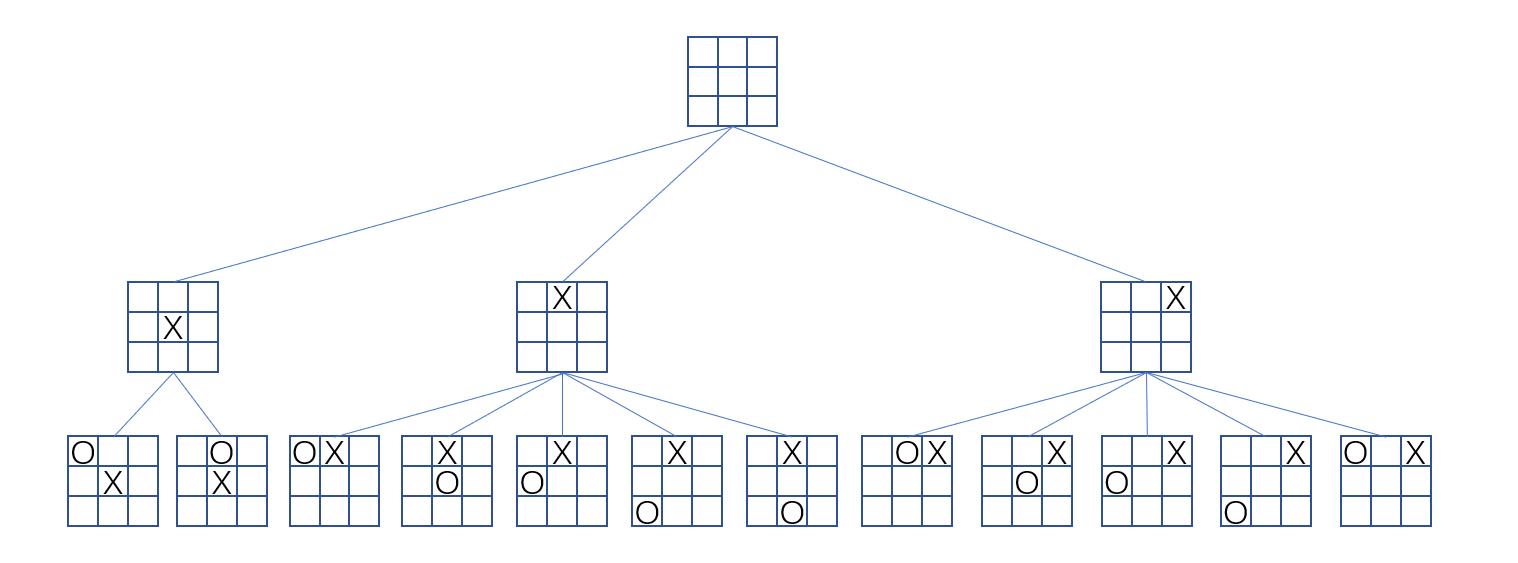
\includegraphics[width=\linewidth]{image/5.9.tree.png}
	\caption{5.9.b game tree starting from an empty board down to depth 2}
\end{figure}\par
\subsection*{c.}
evaluation均已标在图中:
\begin{figure}[H]
	\centering
	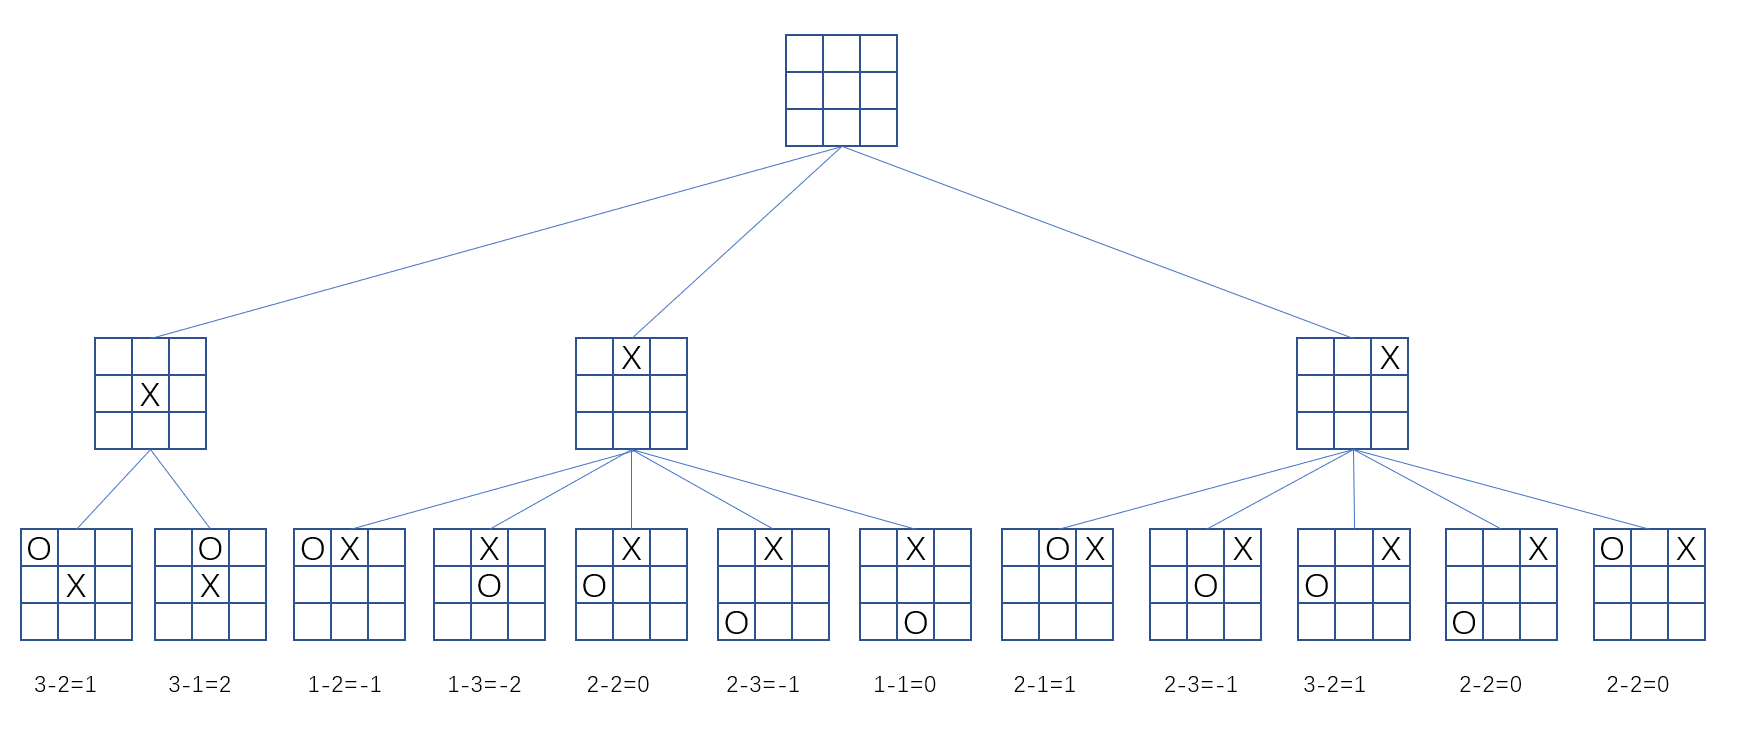
\includegraphics[width=\linewidth]{image/5.9.tree_marked.png}
	\caption{5.9.c marked with evaluations}
\end{figure}\par
\subsection*{d.}
使用 minmax 算法结果如下:
\begin{figure}[H]
	\centering
	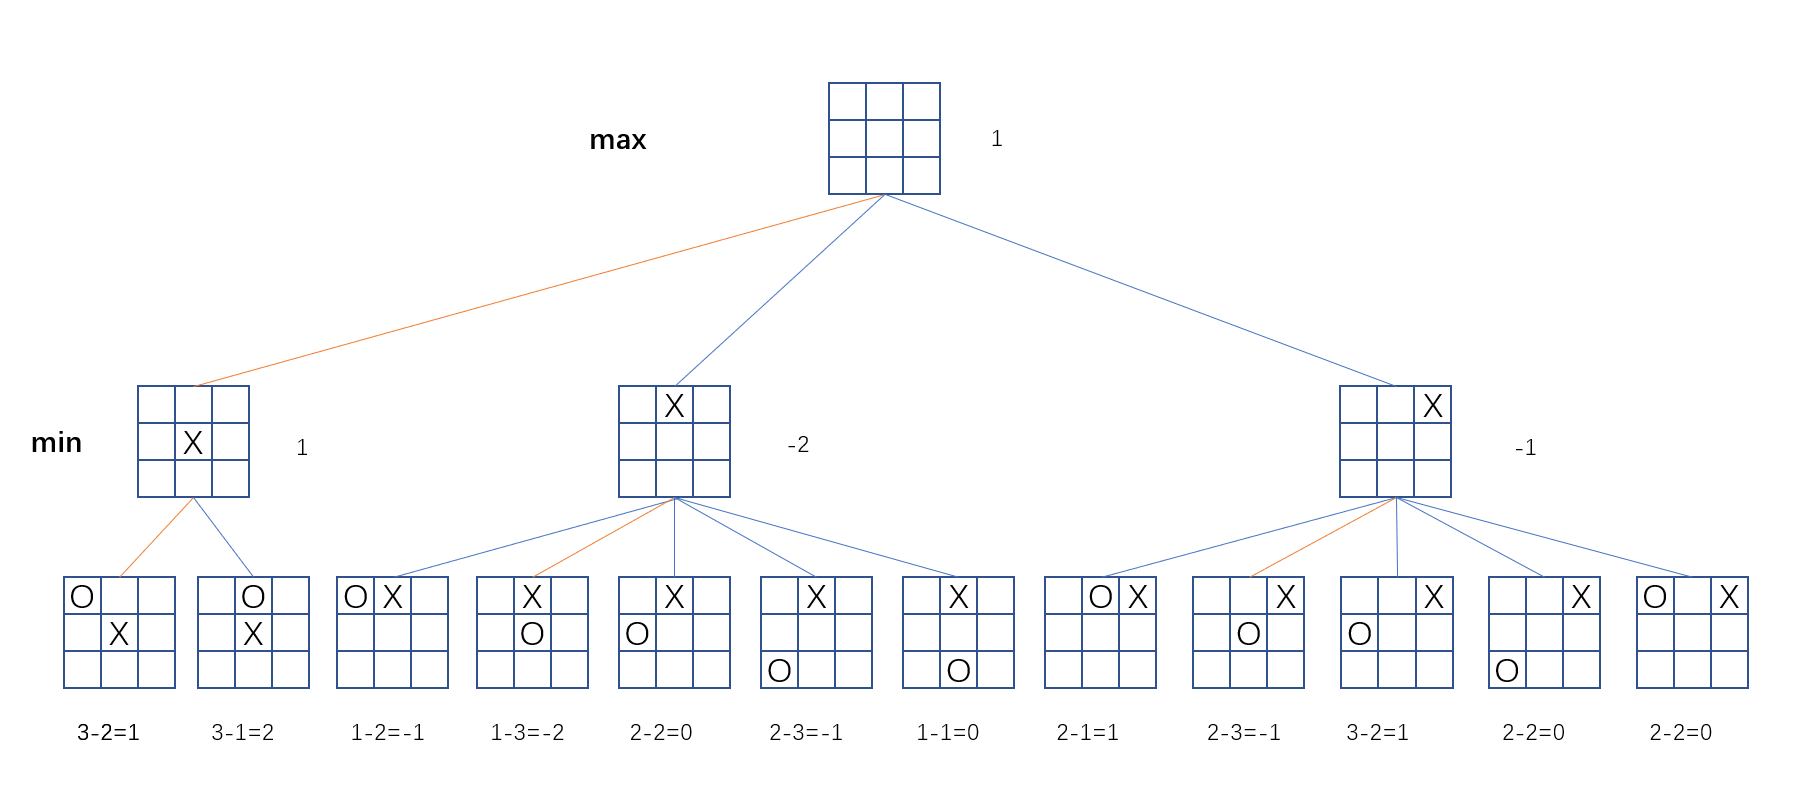
\includegraphics[width=\linewidth]{image/5.9.d.png}
	\caption{5.9.d use minmax algorithm}
\end{figure}\par
因此最佳的初始选择是: 把 X 放在棋盘中间的位置.
\subsection*{e.}
如果顺序是最优的, 那么将会有如下绿色框出的节点不会被测试:
\begin{figure}[H]
	\centering
	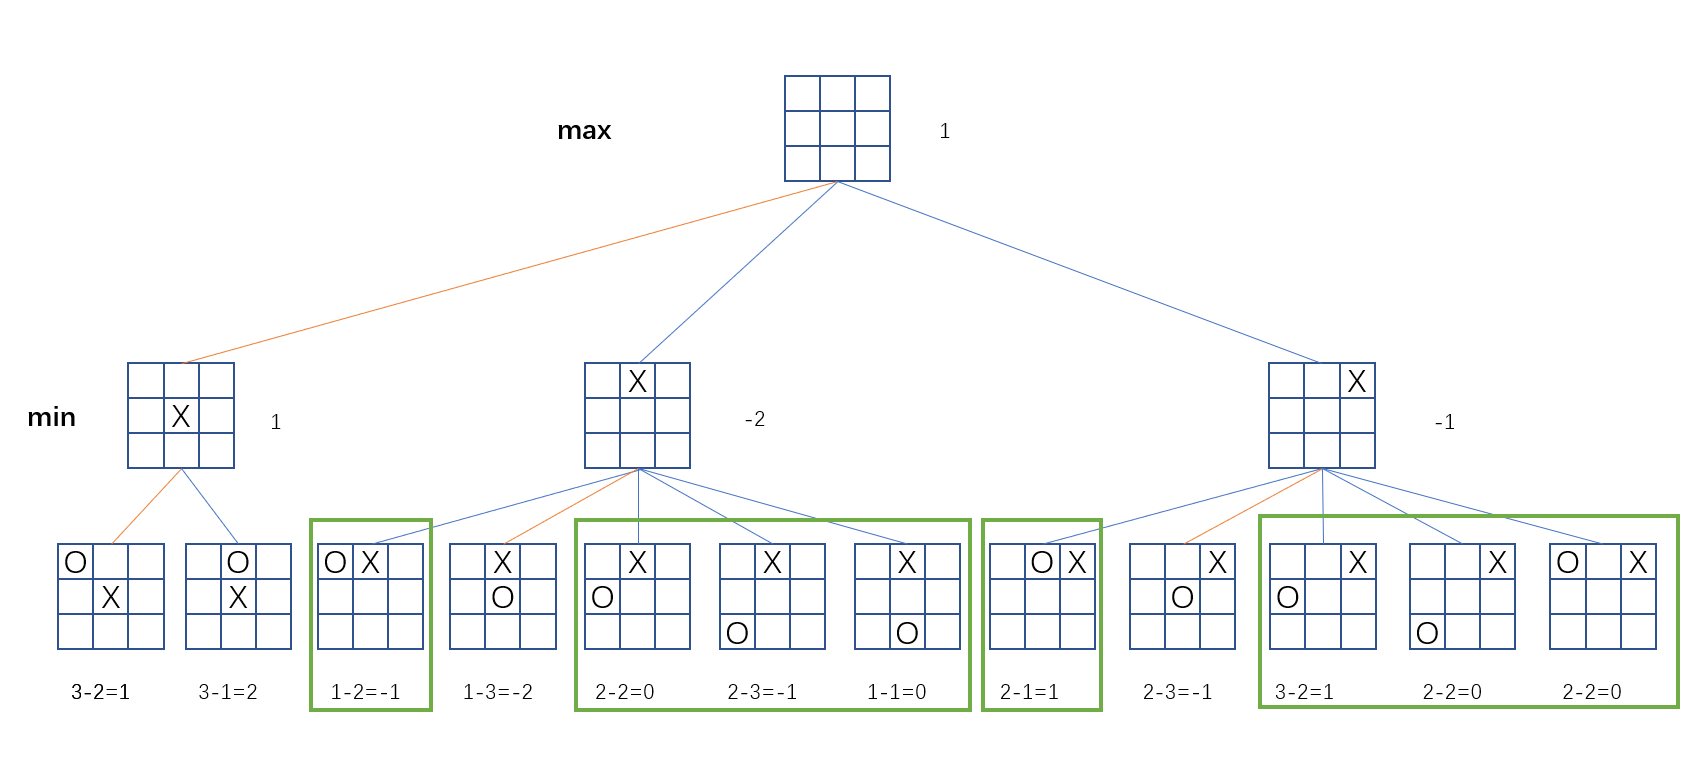
\includegraphics[width=\linewidth]{image/5.9.e.png}
	\caption{5.9.e}
\end{figure}\par

\section*{5.8}
\subsection*{a.}
完整的 game tree 如下图所示:
\begin{figure}[H]
	\centering
	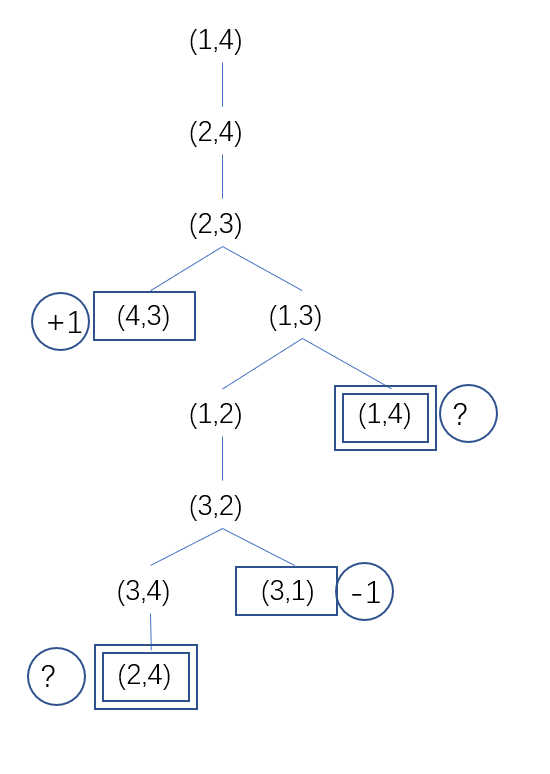
\includegraphics[width=\linewidth/2]{image/5.8.a.png}
	\caption{5.8.a}
\end{figure}\par
\subsection*{b.}
\begin{itemize}
	\item 当面对 +1 和 ? 的时候, 显然选择 +1 的路径能赢, 即 max(+1,?)=+1, min(+1,?)=?
	\item 当面对 -1 和 ? 的时候, 选择 -1 一定不能赢, 但选择 ? 则还有希望能赢, 因此这时要选择 ?, 即 max(-1,?)=?, min(-1,?)=-1
	\item 当面对的子节点只有一个 ?, 就只能选它
	\item 其他组合情况未出现, 故不予定义
\end{itemize}
使用 minmax 算法后如下所示:
\begin{figure}[H]
	\centering
	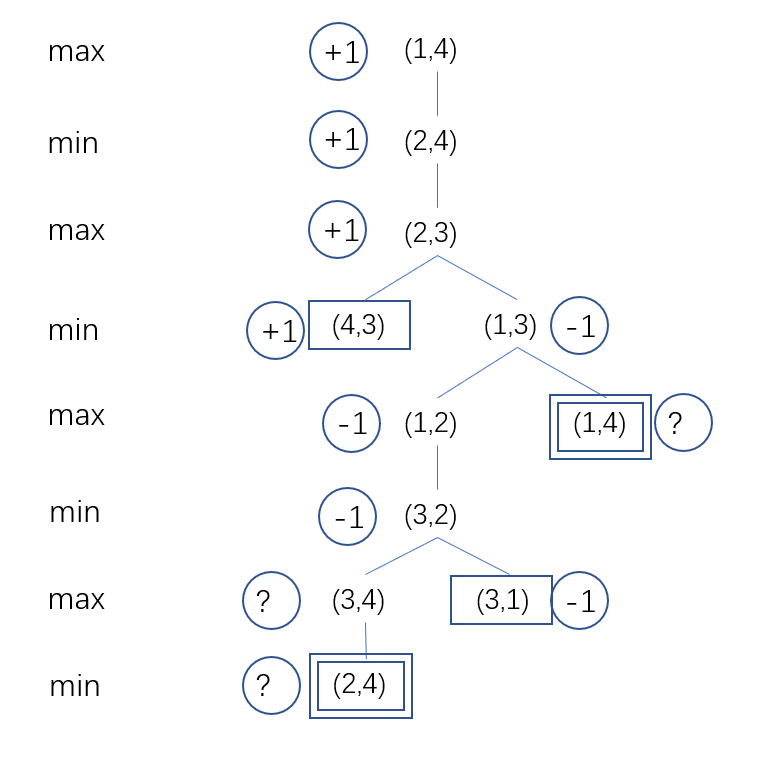
\includegraphics[width=\linewidth/2]{image/5.8.b.png}
	\caption{5.8.b}
\end{figure}\par
\subsection*{c.}
因为运用标准的 minmax 算法会导致陷入死循环. 解决方案是, 将已经访问过的状态放进一个集合里, 每检查一个新节点的时候要首先看一下是否是已经处理过的节点, 如果是的话, 就标记为 ?, 并按 (b) 所述方法处理 ?.

这种方法并不能区分所有带 loop 的游戏, 因为在本题中, loop 出现的时候能够很好地解释 ? 的语义, 并给出应该选择 ? 还是另一个节点, 类似于一种排除法. 但其他游戏则不一定能够精确地定义好 ? 的语义.
\subsection*{d.}
可以考虑数学归纳法
\begin{enumerate}
	\item 据前述, 当 $n = 4$, 先行者胜. 假设 $n \le 2k$ 时, $n$ 为偶数则先行者胜, $n$ 为奇数则后行者胜.
	\item 若 $n = 2k+1$, 则先行者只能有一种走法, 那么变成 $n=2k$ 的情况, 这时, 相当于对手先行的偶数情况, 所以一定是对手胜.
	\item 若 $n=2k+2$, 则先行者走完相当于对手面临 $2k+1$ 的局势, 因为是奇数, 所以对手一定会输, 也就是先行者胜
\end{enumerate}
综上命题得证.

\section*{5.13}
\subsection*{a.}
对于 $n_2$:
$$n_2=\max(n_3,n_{31},\cdots,n_{3b_3})$$
进而 $n_1$ 有:
$$n_1=\min(\max(\min(..., n_{41},n_{4b_4}),n_{31},\cdots,n_{3b_3}), n_{21}, n_{2b_2})$$
其中最内层嵌套的 $\cdots$ 可以不断地用相应的 $n_j$ 替代, 直到最底层 $n_j$.
\subsection*{b.}
则有:
$$n_1=\min(l_2, \max(l_3,...,r_3), r_2)$$
其中最内层嵌套的 $\cdots$ 可以递归地写下去直到最底层的 $\max(l_j,n_j,r_j)$
\subsection*{c.}
\begin{itemize}
	\item 对于极小值($i$ 为偶数)的 $l_i$, 为了让 $n_j$ 有效, 它必须满足 $n_j< l_i$, 否则不如选 $l_i$ 对应的;
	\item 对于极大值($i$ 为奇数)的 $l_i$ 也类似, $n_j>l_i$
\end{itemize}
而 $n_j$ 是一个 max 节点, 因此一定要有 $\max(l_3,l_5,\cdots, l_{j-1})<n_j<\min(l_2,l_4,\cdots, l_{j})$
\subsection*{d.}
则有 $$n_1=\min(l_2, \max(l_3,...,r_3), r_2)$$
其中一直写下去最内层是 $\min(l_j,n_j,r_j)$
从而
\begin{itemize}
	\item 对于极小值($i$ 为偶数)的 $l_i$, 为了让 $n_j$ 有效, 它必须满足 $n_j< l_i$, 否则不如选 $l_i$ 对应的;
	\item 对于极大值($i$ 为奇数)的 $l_i$ 也类似, $n_j>l_i$
\end{itemize}
而 $n_j$ 是一个 max 节点, 因此一定要有 $\max(l_3,l_5,\cdots, l_{j})<n_j<\min(l_2,l_4,\cdots, l_{j-1})$




\end{document}




